\documentclass[a4paper]{article}
\usepackage[margin=50pt]{geometry}
\usepackage{amsmath}
\usepackage{graphicx}
\usepackage{hyperref}
\usepackage{listings}
\usepackage{float}
\usepackage{textcomp}


\lstset{frame=Trbl, numbers=left}
\lstset{
  basicstyle=\ttfamily,
  columns=fullflexible,
  frame=single,
  breaklines=true,
  %postbreak=\mbox{\textcolor{red}{$\hookrightarrow$}\space},
}


\begin{document}
\title{D4 Chinchilla - Team Report}
\author{
Hugo~McNally - hm6g17@soton.ac.uk
\and
Matt Crossley - mac1g17@soton.ac.uk
\and
Matthew Johns - mrj1g17@soton.ac.uk
\and
Mark Warnants - mpw1g17@soton.ac.uk
\and
Francis Wharf - few1g17@soton.ac.uk
\and
William Webb - wcw1g17@soton.ac.uk
\and
Tom Lam - yfl1u17@soton.ac.uk
\and
Kexin Pan - kp1y18@soton.ac.uk
}
\maketitle


\section{Challenge Solution Statement}
The product was conceived to help deaf people navigate day to day conversations
a little easier. Currently, deaf people must follow conversations through the
use of lip reading and following contextual cues. This is made more difficult
when many people talk at once, or don’t get their attention first when talking.
This solution enables deaf people to follow conversations more easily by
visualising the sounds coming towards the listener from around the room, in an
easy to understand way. It also provides a web interface to make interacting
with the device easy, by providing a way to view the current sounds with high
accuracy as well as the history of received sounds. It is easy to set up, and
any firmware updates would be downloaded through the web interface.

This product is a table-top device, enclosed in its own case, with a sleek,
white design. It has a diffused RGB LED ring on top to indicate incoming sounds
as well as their angles, amplitudes and frequencies. It receives its inputs
through four microphones on the top of the device which are sampled and sent to
the system's Raspberry Pi by an ARM microcontroller. Cross correlation and a
fast-fourier transform are carried out on the raspberry pi to extract all the
necessary information out of the incoming signals. A web interface would be
hosted by the Raspberry Pi which provides detailed read outs of all the
information gathered and provides a secure file upload for firmware updates.
There is a hardware calibration button in the centre of the device which,
when pressed, triggers the collection of a ten second sound sample of the
background noise. This is used to determine the level of noise which the device
should subsequently ignore.

The system should be run on a 5 V $\pm$ 400 mV battery with the capability of
driving the whole system with no adverse effects on the operation of the system,
particularly the microphones, pre-amps and analog to digital converters (ADC).
The output of the microphone and pre-amp stages should be between 0 V and 3.3 V.
After going through the ADC stage, it should transmit to the microcontroller in
real-time at 50 Hz. This information should then be buffered on the
microcontroller, and sent to the back-end on the raspberry pi after the data for
that packet of information is collected. This transfer should occur at no less
than 120 kb/s. Analysis will then be carried out in the back-end and an angle of
the sound should be produced to an accuracy of 9\textdegree. An amplitude would also be
produced and frequency information. The resolution of the back-end outputs
should be 8-bits at a frequency of 100 Hz.


\section{System Design}

The purpose of the system was to obtain audio from microphones, extract the
angle of incidence of sounds, and display it on the hardware, and also a web
interface. In order to make this happen, data must be sampled from an analogue
microphone, and processed in a digital form which can be displayed to the user
by some kind of computer. This naturally splits the project into a digital and
analogue component.

For the analogue component of the system, instrumentation amplifiers were
initially chosen to amplify the signal from the microphones, but microphone
pre-amps were later chosen over them, as the microphone output was not
differential, and there were no dual rails.

Four microphones were used, as at minimum three are required to deduce the angle
of a sound, and four microphones simplify the mathematics for calculating
angles. The extra microphone also allows for increased accuracy. Using six or
more was considered, but these ideas were rejected due to the extra hardware
required.

It was also decided to build some analogue filters to remove mains and any other
unwanted noise.  The filtered audio can then be read by ADCs and sent to the
digital components of the system over SPI.

For the digital component of the system, it was decided to use a Raspberry Pi
Model 3, since every member of the team already had one, which would be
exceptionally useful for development and testing. This presents some issues
however. A Pi is well suited to performing the signal processing portion of the
system, as it has a quad-core CPU with multipliers.  However, unless an RTOS is
installed, which would be awkward if it is also running a web server, a
Raspberry Pi cannot sample audio from four separate ADCs at once, with a
consistent sampling rate. It was therefore decided to handle the reading the
ADCs on another piece of hardware.

An FPGA was considered for this role, as in theory it could very rapidly sample
from a set of ADCs, and if one with multipliers was chosen, could even rapidly
perform some of the slower parts of the signal processing.

However, this was rejected in favour of an ARM micro-controller, as a member of
the team already had one to begin development on, and it would cost considerably
less to find the required performance.  Specifically an ARM Development Board
was chosen, as it could easily interface with the Pi over USB to transfer both
data and flash new firmware.

It would be impractical to process data from all four microphones on the
Raspberry Pi in real-time, due to the huge amount of computing power required,
so the decision was taken to buffer the ADCs continually for a period of time
using the micro-controller. The micro-controller can then transfer the raw ADC
readings to the Raspberry Pi over USB serial.

As a user interface, an LED ring was chosen, as it is easy to interpret. It is
also aesthetically pleasing and cheap when compared to a display. A ring of
pre-made addressable LED modules was chosen, as a bespoke solution would have
been unnecessarily complex. The Pi can communicate with the LED ring using the
one-wire protocol.

A web interface was also chosen, as the Pi can easily host a web-server, and it
could be used to upload more firmware to the system, and provide the user more
detailed information.  Finally, a button was also chosen to the Pi, and used to
trigger calibration. The back-end on the Pi could be shut down, or told to
calibrate through a simple downward interface exposed as a FIFO.

\begin{figure}[H]
\begin{center}
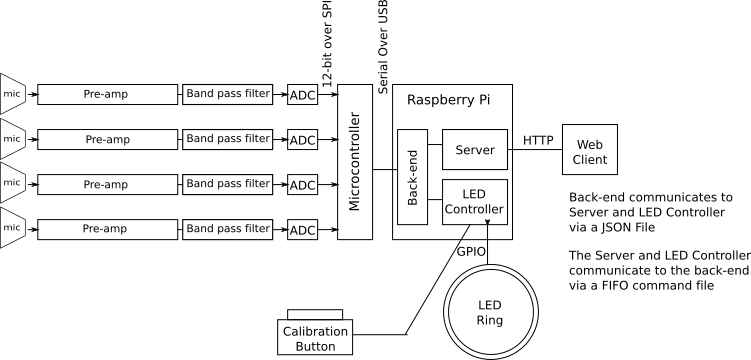
\includegraphics[width=500pt]{appendixC/block_diagram.png}
\caption{block diagram}
\label{fig:blockdia}
\end{center}
\end{figure}

\section{Design Evaluation}

1. Difficulty of specification attempted The specification of this product was
relatively complex. Despite the goal being relatively straightforward, the way
that this was attempted, using multiple microphones and calculating phase
differences of sound signals, required advanced and precise signal processing,
with little room for timing error, as a high sampling rate was necessary to
analyse audio.

2. Quality of the electronic design The design relied heavily on embedded
software, and as a result a lot of the electronics comprised of embedded
development boards. There was realistically no alternative to this in such a
shortage of time. The anti-aliasing filters were second-order, meaning the
roll-off was only 40dB/decade. Given the very narrow range of frequencies audio
occupies, this was not sharp enough to be very effective. A higher order filter
was needed to remove the higher frequencies.  The ADCs were chosen as 13-bit
differential amplifiers, intended to give better common-mode rejection. However,
single-ended ADCs would probably have sufficed, as would a lower resolution,
given only eight bits were used.

3. Ease of use The design was incredibly easy to use as it was designed with
elderly people in mind, as they are the largest demographic for hearing
problems. There was only a single on-off push button for power, and a single
large button on the top for calibration. Audio data was displayed on the LED
ring on the top in an intuitive way.  The case was slightly larger than ideal
when considering portability, but it was not heavy enough to be cumbersome.  The
internals were accessed incredibly easily by rotating the lid a small amount to
release it.

4. Creativity and innovation of the designed product This is a product that we
believe has not yet been brought to market, and is therefore very innovative.
The methods of solving the problem are not revolutionary, but putting them
together in this specific product aimed at improving the lives of people with
hearing problems is a new concept.

5. Aesthetics The case was designed to give it a clean and minimalist look, and
the LEDs were covered by diffuser plastic help the lights blend together in a
smooth, attractive manner. This had the result of our enclosure being one of the
best (if not the best!) looking out of all the teams. The aesthetics were
improved further using LED animations on startup and calibration.

6. Cost Nothing in the device was made of specialist components, and thus
everything was relatively cheap. The major source of cost was the use of the MCU
and Raspberry Pi boards, which would not be used in a production model. They
were also both more powerful than was required for the project, but as exact
performance requirements were not know at the time of design, they were bought
to allow some leeway. Using a plastic case makes the design cheaper to mass
produce.

7. Reliability The design had a calibration feature implemented in software,
which theoretically should allow it to function reliably in most social
environments. Situations in which it may not be reliable include high levels of
vibration of the surface on which it is placed, or if there is a constant, loud
background noise such as heavy machinery. It would not be expected to work
outside unless there was little wind. Tapping the case may reduce reliability
unless padding was introduced between the case and the microphones.  The case is
robust enough to protect the interior electronics during transport and handling.
There is nothing on the outside of the case likely to be broken off.


\section{Quality Factor}

\subsection{Costing}
Appendix [?] contains a breakdown of the costing of the unit. This not only
includes the breakdown of costs associated with producing a single unit but also
the costs incurred with manufacturing the product over a period of time. The
enables the cost of setup fees and development costs to be amortised over a
batch of units, in this case 1000 units, to better estimate a recommended retail
price. A number of assumptions were made, and are stated in appendix [?] that
certain work was done to reduce the price of the unit based on the manufacturing
methods that would be used for a production run of that size.  1000 units was
chosen as it represents a large production run for this product. This is
considering that it is in the accessibility market where it is purchased more
through necessity by a small niche as opposed to being actively market to the
general public as a helpful product.  The recommended retail price here was
estimated to be £405.77. This results in profit of £112.77 per unit sold.

\subsection{Marketing}
As mentioned, the product only appeals to environments where there are a number
of people sitting in static locations. This means the product appeals largely to
conferences in a business setting where a hearing impaired person is involved.
The limits the target audience quite substantially and the best route for
marketing would most probably be through existing companies that already
specialise in accessibility based products such as [?].

\subsection{Conformance Marking}
CE compliance requires the product to visible be marked somewhere on the outer
casing with the official CE logo once conformed. The obvious place for this is
the bottom of the unit. The product would be required to undergo a round of
testing at a verified test house, TUV for example, to ensure it meets
requirements for a number of standards such as radiated, conducted and induced
emissions. Since the product uses wifi for communication, it would have to be
tested under the 'intentional radiator' category which may incur additional cost
or testing over what is in the cost breakdown as in appendix [?]. Quotations
would be necessary to verify this.


\section{Final Product}

First of all, to compare our specification and we have achieved, the back-end
successfully passed all the test by using the test data and it shown it works
for multiple angle with frequency up to 2000Hz. And the back-end we specify that
it needs to be calculated the angle with the tolerance \(\pm 9{^\circ}\). But it
can produce the accuracy of \(0.01{^\circ}\) for a single sine wave. Also, the
microphone can receive the spoken voice and the pre-amp can output the voltage
between 0 to 3.3V from the spoken voice. Moreover, the ADC to MCU communication
can work and sampling the frequency larger than 50kHz. Furthermore, we specify
that the Buffer communicates with Back-end at over 120kB/s.  However, it only
able to communicate at 21.5kB/s. As well as this, the WebUI is able to display
the amplitude and angle of the incoming sound.  In addition, the device is fully
constructed and we are able to put all the components into the case which is
made by a 3D-printer. In terms of the LED ring, we can use it to represent the
signal direction, the frequency and the amplitude by using test data.

In terms of which we cannot achieved, is the WebUI cannot update at a rate
greater than 60fps. And the final device cannot reject artificial ambient noise
and therefore it cannot indicate the correct direction of the signal in a noisy
room.

Next, for our final product, theoretically once an object emitted a sound. The
four microphones inside the device will amplify the sound have been received and
the ADCs which connected to each of the microphones will convert the sound into
a set of real values within a range from 0 to 255. Then it will pass to a
microcontroller and it controls how the data to pass to the Raspberry Pi. Once
the Raspberry Pi received the sets of the real values which come from the
microcontroller, it will compute the program compiled in it. In addition, it
finds the direction of the sound by using cross-correlation and the delay
between 2 signals in order to calculate the angle of the sound that it comes
from. Also, the frequency of the sound is calculated by using the Fourier
Transform. Finally, the device will be able to show the direction of the sound
by turn on the LED light and the frequency of the sound which is represented by
the color of the LED.

Finally, for the further extensions of our device, we would like to add filters
to filter out the frequency which is higher than 12kHz which enable the device
not sampling the signal that we are not in use. Also, we want to use the
frequency to differentiating different sounds from the microphones and improve
the speed and accuracy of LED output.  Furthermore, we want the device able to
sense the position of sounds in absolute space, either distance or magnitude of
the vertical angle.

\begin{figure}[H]
\begin{center}
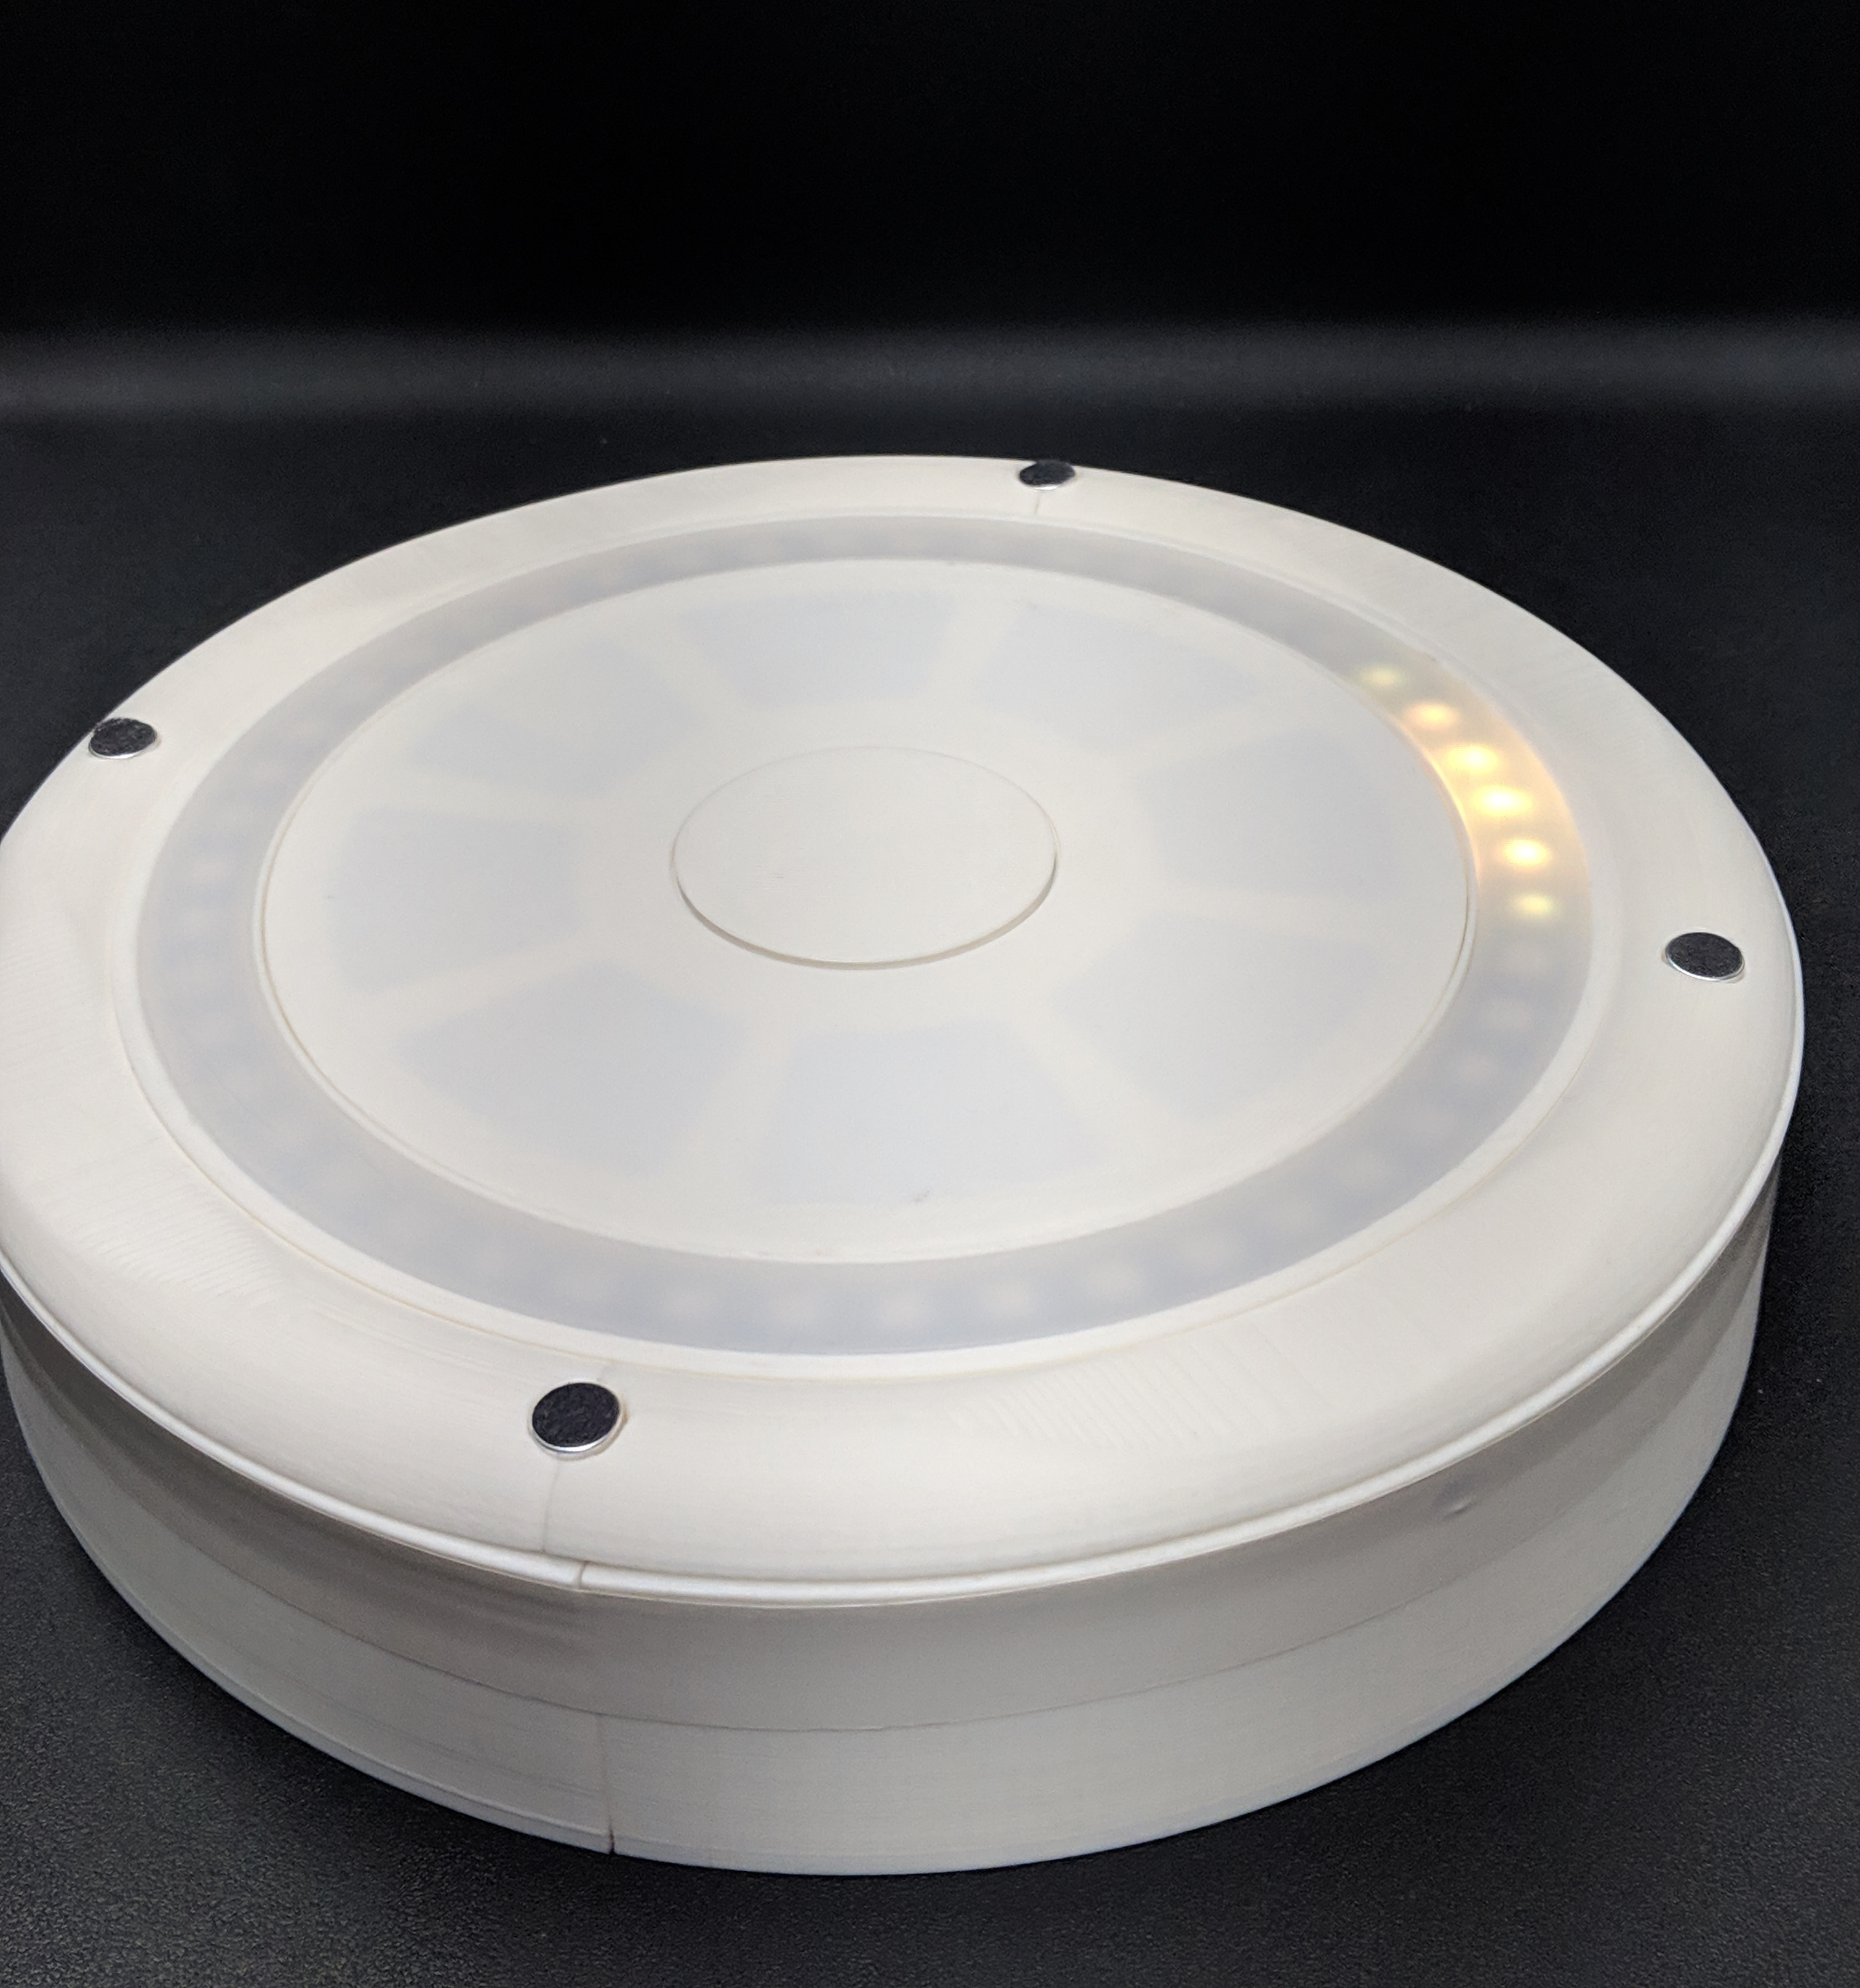
\includegraphics[width=300pt]{pictures/FinalProduct-cropped.jpg}
\caption{Photo of the final product with LED light}
\label{fig:finprod}
\end{center}
\end{figure}


\appendix
\section{Design Completion Form}
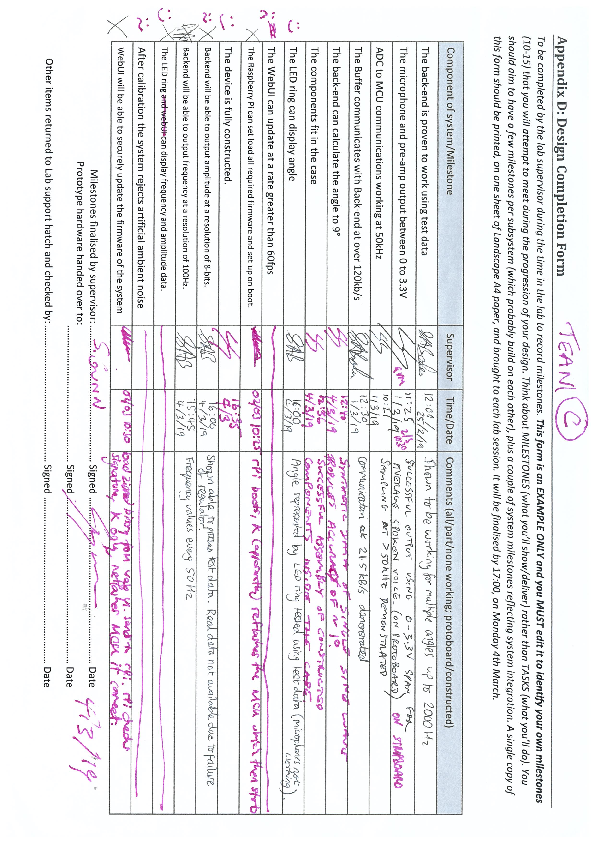
\includegraphics[width=500pt]{appendixA/DesignCompletionForm-complete.png}

\section{Circuit Diagrams}
\begin{figure}[H]
\begin{center}
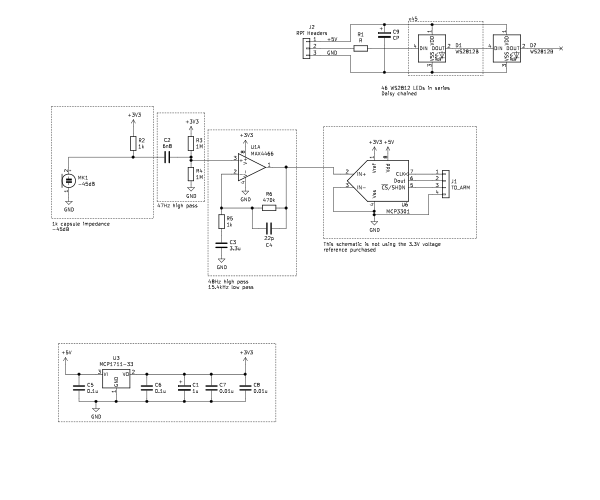
\includegraphics[width=500pt]{appendixC/schematic-cropped.png}
\caption{schematic}
\label{fig:schem}
\end{center}
\end{figure}

\section{Software Listings}

\subsection{Buffer}
% Johns'
arm\_main.cpp
\lstinputlisting[language=c++]{appendixD/code/johns/arm_main.cpp}

logic\_test\_program.cpp
\lstinputlisting[language=c++]{appendixD/code/johns/logic_test_program.cpp}

\subsection{Signal Processing}
% Francis'
conf.h
\lstinputlisting[language=c]{appendixD/code/francis/conf.h}

main.c
\lstinputlisting[language=c]{appendixD/code/francis/main.c}

sample.h
\lstinputlisting[language=c]{appendixD/code/francis/sample.h}

sample.c
\lstinputlisting[language=c]{appendixD/code/francis/sample.c}

sound.h
\lstinputlisting[language=c]{appendixD/code/francis/sound.h}

sound.c
\lstinputlisting[language=c]{appendixD/code/francis/sound.c}

xcorr.h
\lstinputlisting[language=c]{appendixD/code/francis/xcorr.h}

xcorr.c
\lstinputlisting[language=c]{appendixD/code/francis/xcorr.c}

% Tom's
DFT.h
\lstinputlisting[language=c++]{appendixD/code/tom/DFT.h}

DFT.cpp
\lstinputlisting[language=c++]{appendixD/code/tom/DFT.cpp}

backend\_code.cpp
\lstinputlisting[language=c++]{appendixD/code/tom/backend_code.cpp}

dw\_iface.cpp
\lstinputlisting[language=c++]{appendixD/code/tom/dw_iface.cpp}

\subsection{Web}
% Matt's
index.php
\lstinputlisting[language=php]{appendixD/code/matt/index.php}

upload.php
\lstinputlisting[language=php]{appendixD/code/matt/upload.php}

install-daemon.sh
\lstinputlisting[language=bash]{appendixD/code/matt/install-daemon.sh}

% unclaimed
log.js
\lstinputlisting{appendixD/code/unclaimed/log.js}

radar.js
\lstinputlisting{appendixD/code/unclaimed/radar.js}

requestor.js
\lstinputlisting{appendixD/code/unclaimed/requestor.js}

style.css
\lstinputlisting{appendixD/code/unclaimed/style.css}

\subsection{LED Control}
% Mark's
led\_ctl.py
\lstinputlisting[language=Python]{appendixD/code/mark/led_ctl.py}

\end{document}
